\section{System Implementation}

\subsection{Frontend Implementation}

	\subsubsection{Source code structure}

\begin{longtable}{{|m{4.8cm}|m{9.6cm}|}} 
	\hline
	\textbf{Module/component name} & \textbf{Description}\\ \hline
	
	api/ & defines custom instance of api communication instance with the backend server.\\ \hline
	
	assets/ & contains all images and cascading style sheets.\\ \hline
	
	context/ & contains the constants which have to be shared across these components. \\ \hline
	
	hooks/ & contains custom React hooks. \\ \hline
	
	public/ & contains public assets (mostly for landing page). \\ \hline
	
	routes/ & defines all routes of the frontend. \\ \hline
	
	store/ & holds specific states of the frontend. \\ \hline
	
	themes/ & defines the color scheme, palette for the frontend. \\ \hline
	
	utils/ & contains shared utilities across components. \\ \hline
	
	views/ & contains main UI components for each roles. \\ \hline
	
	index.jsx & root component of the frontend. \\ \hline
	
	config.js & contains initial configuration of the front end. \\ \hline
	
	package.json & contains custom scripts and frontend package information. \\ \hline
	
	vite.config.mjs & contains configuration for Vite. \\ \hline
	
	\caption{Frontend source code structure} % needs to go inside longtable environment
	\label{tab:fe-src-code}
\end{longtable}

	
	\subsubsection{UI pages structure}
	These diagrams below illustrate all the Web pages of each role 
	%	Quick brown fox \tikz[baseline=(X.base)]\node [draw=black,fill=cyan!20,thick,rectangle,inner sep=3pt, rounded corners=4pt] (X) {jumped}; over the lazy dog.
	\begin{figure}[H]
		\centering
		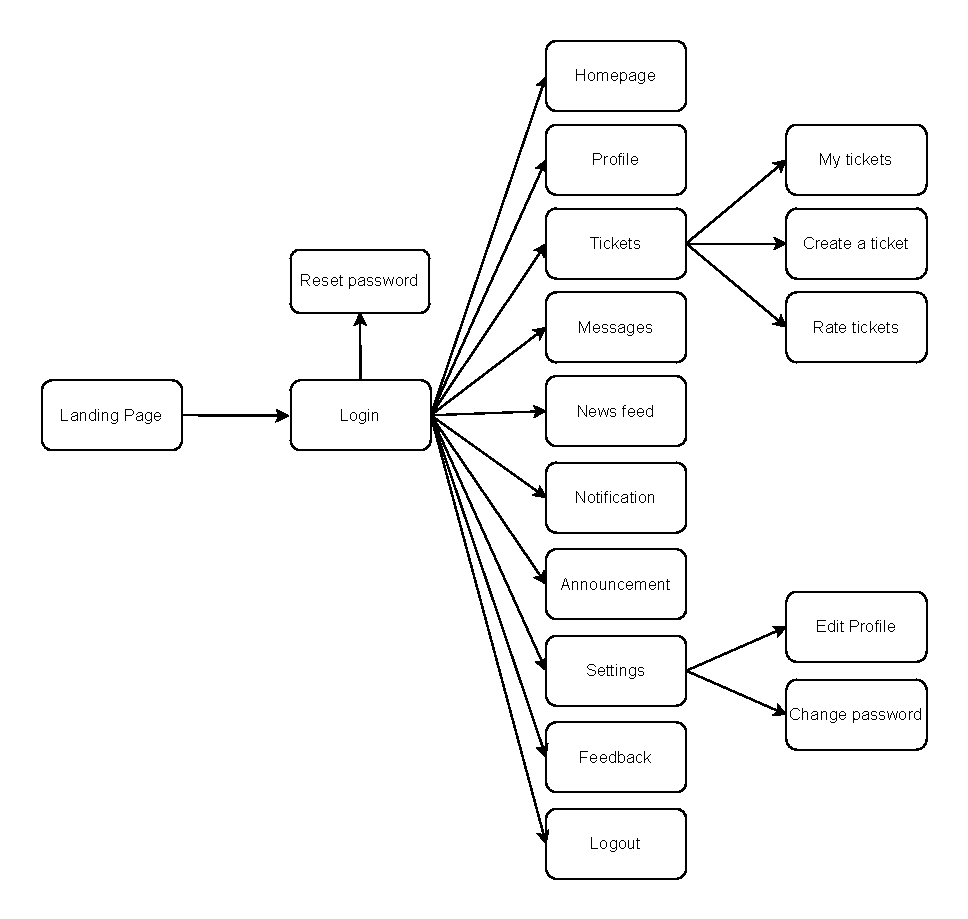
\includegraphics[width=1\linewidth]{graphics/fe/ui-pages-std.pdf}
		\caption{Web UI pages structure of Student role}
		\label{fig:fe-ui-page-std}
	\end{figure}
	
	\begin{enumerate}
		\item \textbf{Landing page}: Students can view the web application overview.
		\item \textbf{Login page}: Students can then enter their credential to access the services.
		\item \textbf{Reset password page}: Students can enter their email to receive the reset password.
		\item \textbf{Homepage}: Students can view the welcome card, guidance, and general personal details
		\item \textbf{Profile}: Students can view their personal details.
		\item \textbf{Tickets}: Students can manage their own tickets.
			\begin{itemize}
				\item \textbf{My ticket}: Student can view all of their tickets.
				\item \textbf{Create a ticket}: Student can create (raise) a new support ticket in the system.
				\item \textbf{Rate tickets}: Student can rate completed support tickets.
			\end{itemize}
		\item \textbf{Messages}: Students can send text messages to the staff who handles the support ticket.
		\item \textbf{News feed}: Students can view all available (pending, in progress) public support tickets in the system.
		\item \textbf{Notification}: Students can view system notifications
		\item \textbf{Announcement}: Students can view system announcements
		\item \textbf{Settings}: 
			\begin{itemize}
				\item \textbf{Edit profile}: Students can modify their personal details.
				\item \textbf{Change password}: Students can change their accounts' password.
			\end{itemize}
		\item \textbf{Feedback}: Students can send their feedback to the system.
		\item \textbf{Logout}: Students can log out of the system.
	\end{enumerate}
	
	\subsubsection{Business Logic}
	

	\subsubsection{UI Main Components}
	\begin{figure}[H]
		\centering
		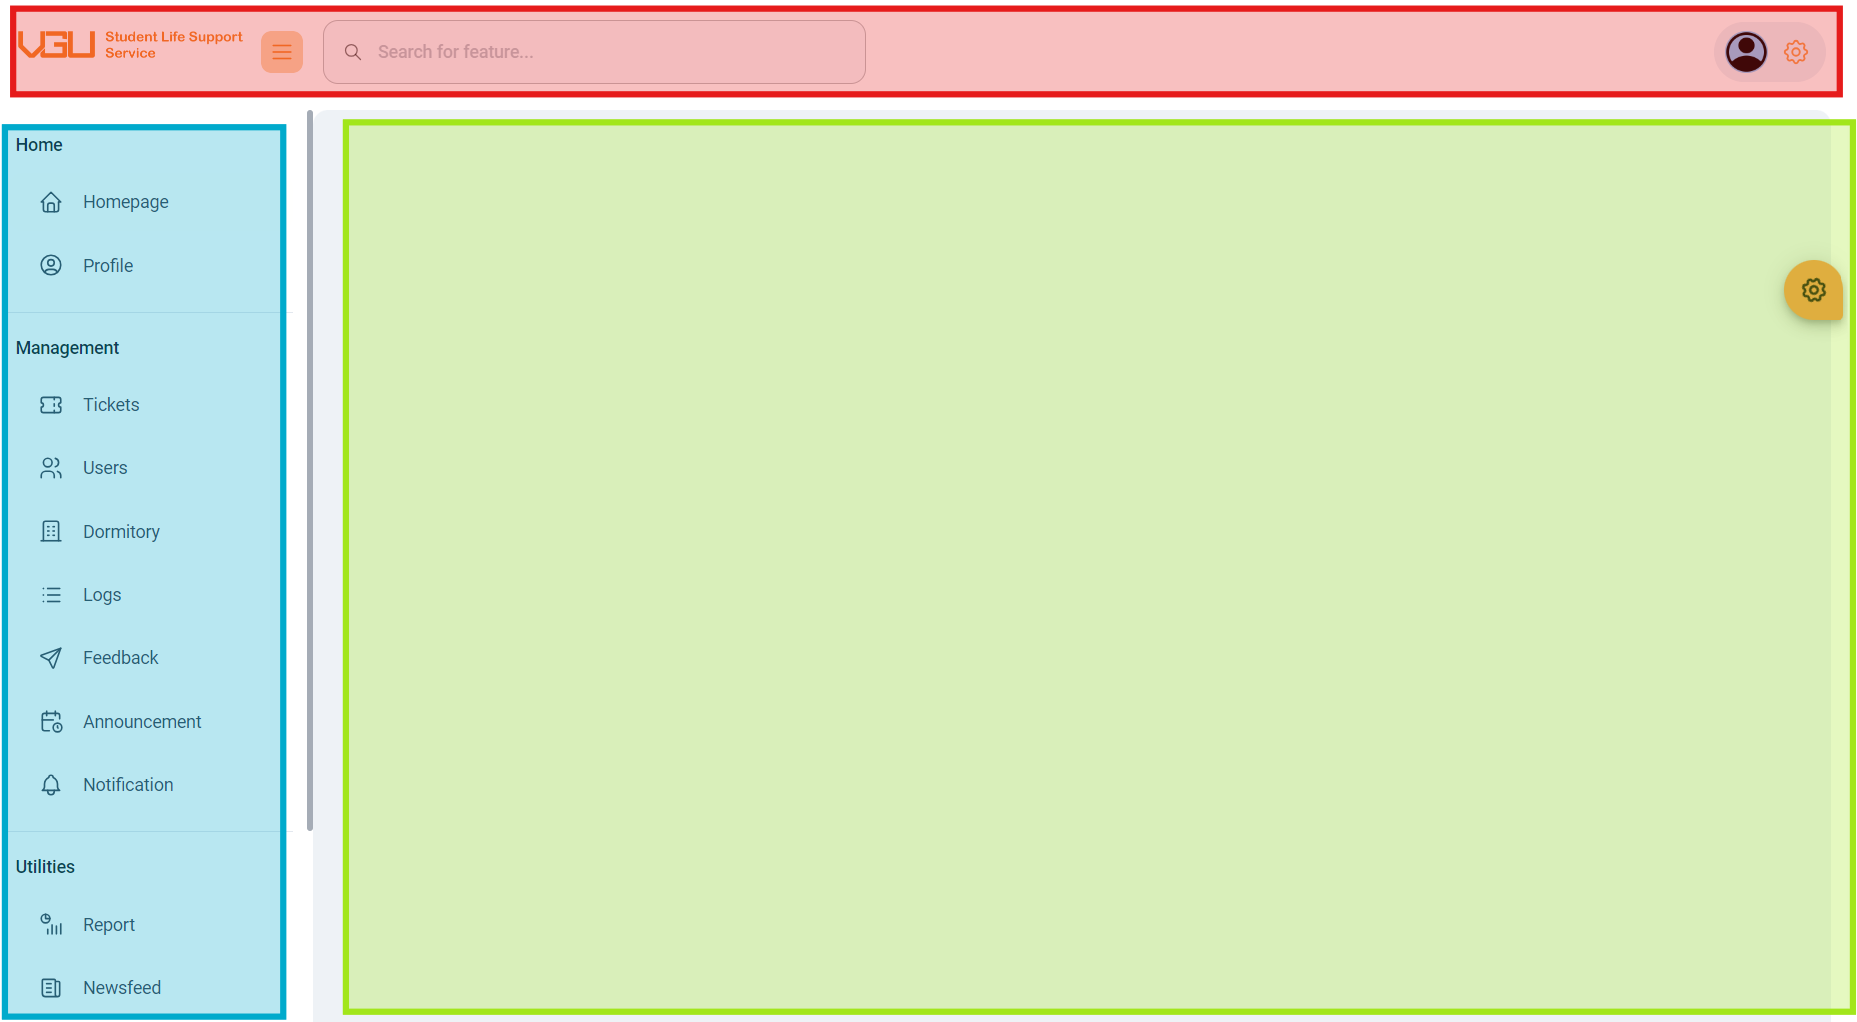
\includegraphics[width=1\linewidth]{graphics/fe/fe-main-comp}
		\caption{Web UI Main Components}
		\label{fig:fe-main-comp}
	\end{figure}
	There are 3 main components in the Web UI (marked on Figure \ref{fig:fe-main-comp}):
	
	\begin{enumerate}
		\item 	\colorbox{Salmon}{Header} (marked as Red color on Figure \ref{fig:fe-main-comp}) contains Logo image, Menu toggle button, Search bar, and Profile section  across all pages
		
\begin{lstlisting}[language=Javascript, breaklines=true, caption=Frontend Header Component]
const Header = ({ handleLeftDrawerToggle }) => {
	const theme = useTheme();
	
	return (
	<>
	{/* logo & toggler button */}
	<Box
	sx={{
			width: 228,
			display: 'flex',
			[theme.breakpoints.down('md')]: {
				width: 'auto'
			}
	}}
	>
	<Box component="span" sx={{ display: { xs: 'none', md: 'block' }, flexGrow: 1 }}>
	<LogoSection />
	</Box>
	<ButtonBase sx={{ borderRadius: '8px', overflow: 'hidden' }}>
	<Avatar
	variant="rounded"
	sx={{
			...theme.typography.commonAvatar,
			...theme.typography.mediumAvatar,
			transition: 'all .2s ease-in-out',
			background: theme.palette.secondary.light,
			color: theme.palette.secondary.dark,
			'&:hover': {
				background: theme.palette.secondary.dark,
				color: theme.palette.secondary.light
			}
	}}
	onClick={handleLeftDrawerToggle}
	color="inherit"
	>
	<IconMenu2 stroke={1.5} size="1.3rem" />
	</Avatar>
	</ButtonBase>
	</Box>
	
	{/* header search */}
	<SearchSection />
	<Box sx={{ flexGrow: 1 }} />
	<Box sx={{ flexGrow: 1 }} />
	

	{/* <ProfileSection /> */}
	<ProfileSection />
	</>
	);
};

Header.propTypes = {
	handleLeftDrawerToggle: PropTypes.func
};

export default Header;
\end{lstlisting}
		
		\item 	\colorbox{Aquamarine}{Sidebar} (marked as Blue color on Figure \ref{fig:fe-main-comp}): A dynamic navigation panel which renders all menu items of a specific roles.
		
\begin{lstlisting}[language=Javascript, breaklines=true, caption=Frontend Sidebar Component]
const Sidebar = ({ drawerOpen, drawerToggle, window }) => {
	const theme = useTheme();
	const matchUpMd = useMediaQuery(theme.breakpoints.up('md'));
	
	const drawer = (
	<>
	<Box sx={{ display: { xs: 'block', md: 'none' } }}>
	<Box sx={{ display: 'flex', p: 2, mx: 'auto' }}>
	<LogoSection />
	</Box>
	</Box>
	
	<BrowserView>
	<PerfectScrollbar
	component="div"
	style={{
			// height: !matchUpMd ? 'calc(100vh - 56px)' : 'calc(100vh - 88px)',
			height: !matchUpMd ? 'calc(100vh - 56px)' : 'calc(100vh - 88px)',
			paddingLeft: '16px',
			paddingRight: '16px'
	}}
	>
	<MenuList />
	{/* <MenuCard /> */}
	<Stack direction="row" justifyContent="center" sx={{ mb: 2 }}>
	<Chip label="v1.0.0" disabled chipcolor="secondary" size="small" sx={{ cursor: 'pointer' }} />
	</Stack>
	</PerfectScrollbar>
	</BrowserView>
	
	<MobileView>
	<Box sx={{ px: 2 }}>
	<MenuList />
	{/* <MenuCard /> */}
	<Stack direction="row" justifyContent="center" sx={{ mb: 2 }}>
	<Chip label="v1.0.0" disabled chipcolor="secondary" size="small" sx={{ cursor: 'pointer' }} />
	</Stack>
	</Box>
	</MobileView>
	
	</>
	);
\end{lstlisting}		
		
		
		
		
		
		\item  \colorbox{YellowGreen}{Content Components} (marked as Green color on Figure \ref{fig:fe-main-comp}): The content component will be displayed based on the matched predefined route. Once the route is determined, the content component is then lazy-loaded into the page. This means that the component will only be fetched and rendered when it is needed, which optimizes performance and improves loading times by minimizing the amount of initial content loaded.
		
		
\begin{lstlisting}[language=Javascript, breaklines=true, caption=Example of Lazy Loading Frontend Components]
const DashboardDefault = Loadable(lazy(() => import('views/homepage')));
const EditProfile = Loadable(lazy(() => import('views/EditProfile')));
const MyTickets = Loadable(lazy(() => import('views/MyTickets')));
\end{lstlisting}	
		
	\end{enumerate}
	
	
	\subsubsection{Responsive Design Implementation}
	Using Material-UI's grid system, responsive components, and utility features enables us to create a flexible and adaptive user interface in React applications. This ensures that the Web UI looks good and functions well on devices of all sizes, enhancing the overall user experience.
	
	\begin{enumerate}
		\item \textbf{Grid System}
		
		MUI provides a powerful Grid component that allows us to create responsive layouts easily. It uses a 12-column layout, and we can specify how many columns a component should span at different screen sizes.


\begin{lstlisting}[language=Javascript, breaklines=true, caption=MUI Grid System]
import { Grid } from '@mui/material';

	<Grid container spacing={2}>
		<Grid item xs={12} sm={6} md={4}>
			<Card>Content 1</Card>
		</Grid>
		
		<Grid item xs={12} sm={6} md={4}>
			<Card>Content 2</Card>
		</Grid>
	
		<Grid item xs={12} md={4}>
			<Card>Content 3</Card>
		</Grid>
	</Grid>
\end{lstlisting}		

	\item \textbf{Media Queries}
	
	MUI allows us to utilize CSS media queries through the sx prop or styles to create responsive designs that adapt to different screen sizes without much hassle.

\begin{lstlisting}[language=Javascript, breaklines=true, caption=MUI Media Queries]
<Box sx={{ 
		display: { xs: 'block', sm: 'flex' }, 
		flexDirection: { xs: 'column', sm: 'row' } 
}}>
{/* Our content */}
</Box>

\end{lstlisting}	


	\end{enumerate}
	
	
\newpage
\subsection{Backend Implementation}
	\subsubsection{Source code structure}
	
	\begin{longtable}{{|m{4.8cm}|m{9.6cm}|}} 
		\hline
		\textbf{Module/component name} & \textbf{Description}\\ \hline
		
		config/ & contains server configurations, database connection class, constants.\\ \hline
		
		controllers/ & contains API controllers.\\ \hline
		
		middleware/ & contains server middleware (token authentication, logger, mailer). \\ \hline
		
		routes/ & defines explicit API routes.  \\ \hline
		
		sql/ & contains all SQL queries. \\ \hline
		
		uploads/ & saves the user's uploaded attachments.\\ \hline
		
		utils/ & contains shared utilities across modules. \\ \hline
		
		index.js & root (start module) module of the backend server. \\ \hline
		
		package.json & contains custom scripts and backend packages information. \\ \hline
		
		.env & contains sensitive backend configurations. \\ \hline
		
		\caption{Backend source code structure} % needs to go inside longtable environment
		\label{tab:be-src-code}
	\end{longtable}
	
	
	\subsubsection{Setting up ExpressJs Server}
	The implementation below sets up a web server with essential middleware and route handling for a robust application. It initializes the app, enabling JSON parsing, cookie parsing, and Cross-Origin Resource Sharing (CORS) with restricted options. The server then defines various API endpoints for authentication and resource management, including user, dorm, ticket, attachment, rating, message, role, notification, announcement, feedback, logs, and reports. Each route corresponds to a specific functionality, organized under the /auth and /api/v1/ prefixes, ensuring a structured and scalable approach to managing the application’s various services.

\begin{lstlisting}[language=Javascript, breaklines=true, caption=ExpressJS Server Setup]
const app = express();
app.use(express.json());
app.use(cookieParser()); // Enable cookie parsing
app.use(cors(WebConfig.corsOptions));


// ==============================|| Routes ||============================== //
app.use("/auth", authRoutes);                     
app.use("/api/v1/users", userRoutes);                  
app.use("/api/v1/dorms", dormRoutes)
app.use("/api/v1/tickets", ticketRoutes);        
app.use("/api/v1/attachments", attachmentRoutes); 
app.use("/api/v1/rating", ratingRoutes);          
app.use("/api/v1/messages", messageRoutes);
app.use("/api/v1/roles", roleRoutes);       
app.use("/api/v1/notification", notificationRoutes); 
app.use("/api/v1/announcement", announcementRoutes);        
app.use("/api/v1/feedback", feedbackRoutes);       
app.use("/api/v1/logs", logsRoutes);     
app.use("/api/v1/reports", reportRoutes);
\end{lstlisting}	

	\subsubsection{Database Integration}
	
\begin{lstlisting}[language=Javascript, breaklines=true, caption=Server connects to PostgreSQL Database]
import pkg from 'pg';
import dotenv from 'dotenv';

dotenv.config();

const { Pool } = pkg;

const pool = new Pool({
	user: String(process.env.PG_DB_USER),
	host: String(process.env.PG_DB_HOST),
	password: String(process.env.PG_DB_PASSWORD),
	port: Number(process.env.PG_DB_PORT),
	database: String(process.env.PG_DB_DATABASE),
});

export default pool;  
\end{lstlisting}	


\begin{lstlisting}[language=Javascript, breaklines=true, caption=Server connects to Redis]
import redis from 'redis';

const redisClient = redis.createClient({
	socket: {
		host: process.env.REDIS_HOST,
		port: process.env.REDIS_PORT,
	},
});


const connectRedis = async () => {
	await redisClient.connect();
	redisClient.on('error', (err) => {
		console.error('Redis error:', err);
	});
	console.log('Redis connected successfully');
};
\end{lstlisting}	


\subsubsection{Middleware}
In the system, the \texttt{authenticateToken} middleware is designed to protect API endpoints by verifying JWT (JSON Web Tokens) based on user roles. The authenticateToken function accepts an array of allowedRoles, which specifies which user roles are permitted to access the route that this middleware protects. The middleware checks for a valid access token in the request headers and verifies it against predefined secrets corresponding to different user roles (e.g., student, staff, admin).

Additionally, \texttt{logger} - an asynchronous middleware designed to log events to a PostgreSQL database. This function serves as a logging mechanism, capturing important user actions or system events and storing them in a dedicated "Log" table. 
\begin{lstlisting}[language=Javascript, breaklines=true, caption= Logger middleware - write log to database]
const writeLogToDB = async (user_id, event_id, description, timestamp) => {
	try {
		await pool.query('BEGIN');
		await pool.query(
		'INSERT INTO "Log" (user_id, event_id, description, timestamp) VALUES ($1, $2, $3, $4)',
		[user_id, event_id, description, timestamp]
		);
		await pool.query('COMMIT');
		logger.info('Log written to database');
	} catch (error) {
		await pool.query('ROLLBACK');
		logger.error(error);
	}
};
\end{lstlisting}	

\subsubsection{Real-time messages}
By creating an HTTP server that integrates with the existing Express application. The Socket.IO server is attached to this HTTP server, allowing for real-time communication over web sockets.

\begin{lstlisting}[language=Javascript, breaklines=true, caption=Create Socket.io HTTP server]
const server = http.createServer(app);
const io = new Server(server, {
	cors: {
		origin: WebConfig.corsOptions.origin,
		methods: ['GET', 'POST'],
	},
});
\end{lstlisting}	



The backend sets up an event listener for incoming connections using the \texttt{io.on('connection')} method. This function is triggered whenever a new user connects to the server. When a user joins a conversation, they emit a \texttt{join\_conversation} event along with the \texttt{ticket\_id} of the conversation.

\begin{lstlisting}[language=Javascript, breaklines=true, caption=Socket.io join\_conversation event]
socket.on('join_conversation', (ticket_id) => {
	socket.join(ticket_id);
	console.log(`User joined conversation ${ticket_id}`);
});
\end{lstlisting}	

When a user sends a message, they emit a \texttt{send\_message} event with the message details. This event is processed to store the message in the database and then broadcast it to other users in the same conversation.


\begin{lstlisting}[language=Javascript, breaklines=true, caption=Socket.io send\_message event]
socket.on('send_message', async (data) => {
	const { ticket_id, sender_id, message_details } = data;
	const created_date = new Date();
	
	try {
		await pool.query('BEGIN'); // Start a transaction
		
		// Insert messages data into database
		
		await pool.query('COMMIT'); // Commit the transaction
		
		io.to(ticket_id).emit('receive_message', newMessage); // Emit the new message to the room
	} catch (err) {
		await pool.query('ROLLBACK'); // Rollback in case of error
		console.error(err);
	}
});

\end{lstlisting}	

Lastly, the disconnect event is implemented to clean up and log when a user disconnects from the conversation.
\begin{lstlisting}[language=Javascript, breaklines=true, caption=Socket.io disconnect event]
socket.on('disconnect', () => {
	console.log('A user disconnected from the conversation');
	// Handle clean up
});
\end{lstlisting}

\newpage
\subsection{Security Measures}
	\subsubsection{JWT Authentication/Authorization}
	\begin{figure}[H]
		\centering
		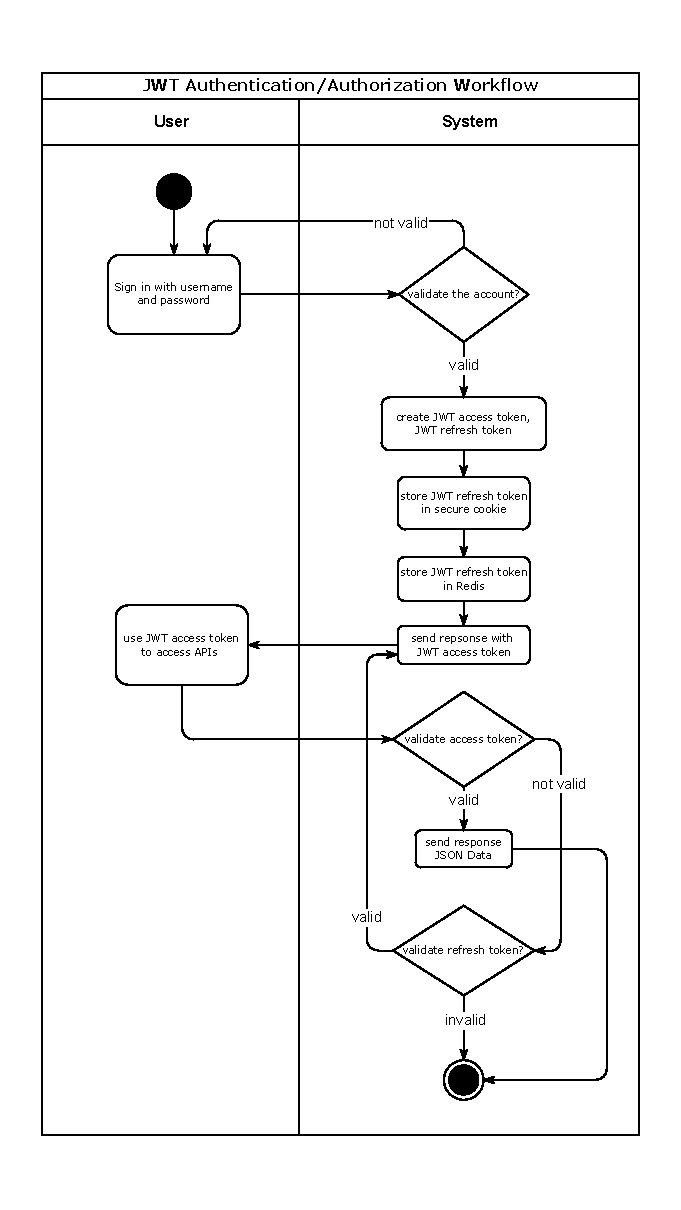
\includegraphics[width=0.58\columnwidth]{graphics/jwt-auth.pdf}
		\caption{JWT Authentication/Authorization Workflow}
		\label{fig:jwt-auth}
	\end{figure}
	
	The JWT (JSON Web Token) authentication and authorization workflow in the Student Life Support Service is designed to ensure secure access to the system's resources while providing a seamless user experience. The process begins when a user signs in by submitting their credentials, such as a username and password. Upon successful validation of these credentials, the system generates two tokens: an access token and a refresh token. The access token is used for short-term authorization and is typically included in the Authorization header of API requests to grant the user access to protected resources. 
	
	\noindent To ensure a high level of security, the refresh token is stored in two secure locations: a cookie on the client-side and in Redis, which serves as an in-memory database for managing sessions. The refresh token allows the system to issue a new access token when the original one expires, ensuring that the user does not need to log in repeatedly.
	
	\noindent When a user makes an API request, the system first checks the validity of the provided access token. If the token is valid, the request is processed, and the appropriate data is returned. However, if the access token is expired or invalid, the system turns to the refresh token. If the refresh token is verified as valid, a new access token is generated, and the user can continue to access the API without re-authenticating.
	
	\noindent In cases where both the access and refresh tokens are invalid, the user is required to log in again, ensuring that expired or tampered tokens do not grant unauthorized access to the system. By utilizing this access-refresh token structure, with refresh tokens stored securely in Redis and cookies, the system balances both security and usability, providing users with continuous access while protecting against unauthorized usage or token expiration.
	
	\noindent This approach ensures that the system is scalable and can handle multiple user sessions efficiently, while also offering robust security through token validation and management.

\begin{lstlisting}[language=Javascript, breaklines=true, caption=Store refresh token in secure cookie]
// Send Refresh Token as an HTTP-only, Secure cookie
res.cookie('refreshToken', refreshToken, {
	httpOnly: true,       					// Prevent JavaScript access to the cookie
	secure: true,         					// Send only over HTTPS
	sameSite: 'Strict',   					// Protect against CSRF
	maxAge: REFRESH_TOKEN_EXPIRED_IN * 1000, 
});
\end{lstlisting}

	\subsubsection{Password Hashing}
	All user passwords within the system are securely protected through the use of a one-way hashing algorithm. This is accomplished by employing the \texttt{\textbf{bcryptjs}} library, which ensures that passwords are irreversibly encrypted, thereby enhancing the security and integrity of user credentials. \\
	
	The \texttt{\textbf{hashPassword}} function below takes a user's plaintext password as input and securely hashes it. First, the function generates a salt using bcrypt.genSalt, which adds an extra layer of randomness to the hashing process. This salt is combined with the user's password using the bcrypt.hash function to create a unique hashed version of the password. The hashed password is then returned, ensuring that even if the same password is used by multiple users, the stored hash will be different due to the unique salt for each password. In case of any errors during this process, the function throws a detailed error message for debugging purposes.
	
\begin{lstlisting}[language=Javascript, breaklines=true, caption=Password Hashing]
async function hashPassword(userInputPassword) {
	try {
		const salt = await bcrypt.genSalt(saltRounds);
		const hash = await bcrypt.hash(userInputPassword, salt);
		return hash; // Return the hashed password
	} catch (error) {
		throw new Error('Error hashing password: ' + error.message);
	}
}
\end{lstlisting}

	The verifyPassword function is used to check if a user's inputted password matches the stored hashed password in the system. It does this by using bcrypt.compare, which compares the plaintext password with the hashed password stored in the database. If the passwords match, the function returns true; otherwise, it returns false. Similar to hashPassword, if an error occurs during the verification process, an error message is thrown for further investigation.
	
\begin{lstlisting}[language=Javascript, breaklines=true, caption=Password Verification]
async function verifyPassword(userInputPassword, encryptedPassword) {
	try {
		const isMatch = await bcrypt.compare(userInputPassword, encryptedPassword);
		return isMatch;
	} catch (error) {
		throw new Error('Error verifying password: ' + error.message);
	}
}
\end{lstlisting}
	
	
	
	\subsubsection{Google reCAPTCHA}
	Google reCAPTCHA is a security service designed to protect websites from bots and automated abuse. It uses a combination of behavioral analysis, machine learning, and user challenges to distinguish between human users and malicious bots. The main goal of reCAPTCHA is to prevent attacks such as credential stuffing, brute-force attempts, and other forms of automated exploits while allowing legitimate users to interact with the site without interruption. \cite{google-recaptcha}
	
	In this system, integrating reCAPTCHA in the "Edit Profile" and "Change Password" features enhances security by preventing automated attacks and brute-force attempts. It ensures that only legitimate users can make critical changes, reducing the risk of unauthorized access and data breaches. reCAPTCHA also helps protect sensitive user information, adds an extra layer of verification for critical actions, and prevents abuse or spam, maintaining system integrity and keeping accounts secure.
	\begin{figure}[H]
		\centering
		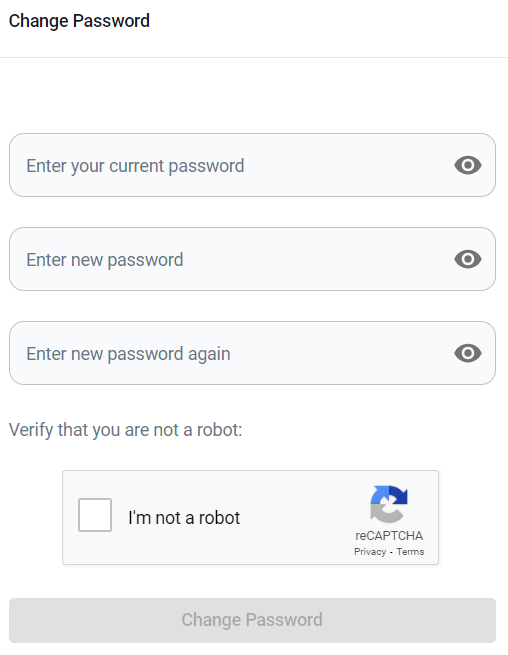
\includegraphics[width=0.3\linewidth]{graphics/change-password-captcha}
		\caption{reCAPTCHA in Change Password form}
		\label{fig:change-password-captcha}
	\end{figure}
	
	
	
	
	
	